%% Part 2.1 calculi fragment: v1.1 Part II, lines 2187--2450, plus
%% D-P2-001 and the propositional half of D-P3-002.  Rules occur only in the
%% registry sheets named below.  Apparatus: A-031, A-115--A-117, A-120.

\section{Classical propositional calculi}
\label{sec:p02-propositional-calculi}

Four presentations are used here: natural deduction, two-sided sequents,
a Hilbert calculus, and analytic tableaux.  Their rule displays live only in
the registry.  Natural deduction uses
\hyperref[sheet:nd-cpl]{\texttt{sheet:nd-cpl}}, and sequents use
\hyperref[sheet:lk]{\texttt{sheet:lk}}; the new entries use
\hyperref[sheet:hilbert-cpl]{\texttt{sheet:hilbert-cpl}} and
\hyperref[sheet:tableaux-cpl]{\texttt{sheet:tableaux-cpl}}.  The first two
are the v1.1 calculi; the new entries fill D-P2-001 and the propositional half
of D-P3-002.  The natural-deduction and sequent presentations use
\cite{Gentzen1934a,Kleene1952}; the Hilbert entry uses \cite{Mendelson1997},
and the tableau entry uses \cite{Smullyan1968}.

\subsection{Natural deduction}
\label{sec:p02-natural-deduction}

\begin{hbdefinition}{def:p02-nd-derivation}{Natural-deduction derivation}
A \emph{natural-deduction derivation} in
\(\mathsf{ND}_{\mathsf{CPL}}\) is a finite rooted tree generated by the
registry sheet \hyperref[sheet:nd-cpl]{\texttt{sheet:nd-cpl}}.  Its leaves are assumption
occurrences.  Discharge labels are metalinguistic markers in \(\mathbb N\),
not symbols of a formula.  An assumption occurrence is \emph{open} exactly
when no rule application on its path to the root discharges its label.

An application of implication introduction, negation introduction, or
reductio carries one label and discharges exactly all open occurrences of its
displayed assumption bearing that label above its premise.  Disjunction
elimination carries two labels and performs the corresponding discharge in
its two minor subderivations.  Each carried label must mark at least one such
open occurrence: vacuous discharge is not licensed.

Consistently and injectively renaming the assumption labels and matching rule
labels preserves both the derivation and its discharge relation.  Because a
derivation is finite, every inserted copy can be renamed to a label set
globally fresh from the receiving derivation and from all other copies.
Several open occurrences of one formula may instead be given one common
fresh label when a newly added root inference is to discharge all of them;
this merging relabeling is not an injective renaming.  There is no repetition
rule: when one premise is needed in two branches, the tree has two assumption
occurrences; no inference duplicates an already derived node.
\end{hbdefinition}

\begin{hbdefinition}{def:p02-nd-derivability}{Propositional natural-deduction derivability}
For \(\Gamma\subseteq\mathsf{Fm}_{\mathsf{CPL}}\),
\[
 \Gamma\derives_{\mathsf{ND}_{\mathsf{CPL}}}\varphi
\]
means that a \(\mathsf{ND}_{\mathsf{CPL}}\)-derivation of \(\varphi\)
exists whose every open assumption belongs to \(\Gamma\).  A proof is the
finite derivation together with its stated set of permitted open assumptions;
the set may contain formulas not used by the derivation.
\end{hbdefinition}

\begin{hblemma}{thm:p02-nd-open-substitution}{proved=annex:p2.calc.1}{Substitution for open assumptions}
Let \(D\) be a natural-deduction derivation of \(\psi\), choose any family
of its open occurrences of \(\varphi\), and let \(E\) be a derivation of
\(\varphi\).  Replace every chosen occurrence by a copy of \(E\), after
consistently renaming every label in each copy to be globally fresh from
\(D\) and from every other copy.  The resulting tree is a derivation of
\(\psi\).  Its open assumptions are exactly the unreplaced open occurrences
of \(D\), together with the correspondingly renamed open assumptions of all
inserted copies of \(E\).
\end{hblemma}

\begin{figure}[htbp]
\centering
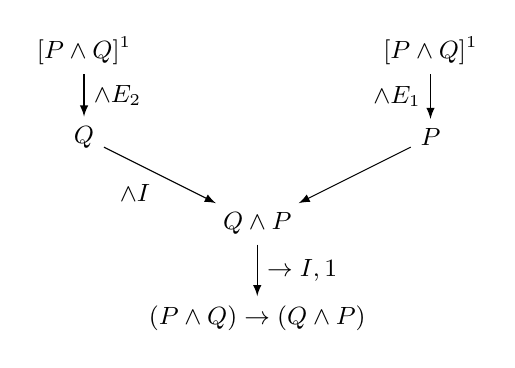
\begin{tikzpicture}[font=\small,>=latex]
  \node (a1) at (-2.2,3.2) {$[P\land Q]^1$};
  \node (a2) at ( 2.2,3.2) {$[P\land Q]^1$};
  \node (q)  at (-2.2,2.1) {$Q$};
  \node (p)  at ( 2.2,2.1) {$P$};
  \node (qp) at (0,1.0) {$Q\land P$};
  \node (imp) at (0,-0.2) {$(P\land Q)\to(Q\land P)$};
  \draw[->] (a1) -- node[right] {$\land E_2$} (q);
  \draw[->] (a2) -- node[left] {$\land E_1$} (p);
  \draw[->] (q) -- node[below left] {$\land I$} (qp);
  \draw[->] (p) -- (qp);
  \draw[->] (qp) -- node[right] {$\to I,1$} (imp);
\end{tikzpicture}
\caption{A complete natural-deduction tree for conjunction commutativity
(A-115).  The two top nodes are assumption occurrences, not repetition
inferences; the final inference nonvacuously discharges both open occurrences
marked \(1\).}
\label{fig:p02-nd-tree}
\end{figure}

\subsection{Finite-multiset sequents}
\label{sec:p02-sequents}

\begin{hbdefinition}{def:p02-finite-multiset-sequent}{Finite multiset and sequent}
A \emph{finite multiset of propositional formulas} is a function
\(\Gamma:\mathsf{Fm}_{\mathsf{CPL}}\to\mathbb N\) with finite support
\[
 \operatorname{supp}(\Gamma)
 \defeq\{\varphi\in\mathsf{Fm}_{\mathsf{CPL}}:\Gamma(\varphi)>0\}.
\]
The empty multiset is the constant-zero function.  A comma denotes pointwise
sum; a displayed formula denotes its singleton multiset.  Thus
\(\Gamma,\varphi,\varphi\) adds two to the multiplicity of \(\varphi\).

A \emph{sequent} is \(\Gamma\Rightarrow\Delta\) for finite multisets
\(\Gamma,\Delta\).  A valuation satisfies it exactly when some formula in
\(\operatorname{supp}(\Gamma)\) is false or some formula in
\(\operatorname{supp}(\Delta)\) is true.  Hence an empty antecedent behaves
as \(\topv\) and an empty succedent as \(\bottom\).  Multiplicity is
proof-structural data in \(\mathsf{LK}\); semantic consequence and
natural-deduction assumptions depend only on support.  In particular, when a
finite multiset appears to the left of \(\entails\) or of a single-conclusion
\(\derives\), it abbreviates its support.
\end{hbdefinition}

The propositional restriction of registry sheet
\hyperref[sheet:lk]{\texttt{sheet:lk}} is the
active \(\mathsf{LK}_{\mathsf{CPL}}\): two-sided finite-multiset sequents,
contexted initial sequents, primitive negation, and exchange built into the
multiset representation.  The sheet alone displays its structural, logical,
and cut rules.

\begin{figure}[htbp]
\centering
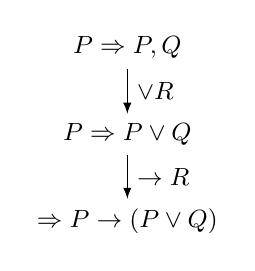
\begin{tikzpicture}[font=\small,>=latex]
  \node (id) at (0,2.2) {$P\Rightarrow P,Q$};
  \node (orr) at (0,1.1) {$P\Rightarrow P\lor Q$};
  \node (impr) at (0,0) {$\Rightarrow P\to(P\lor Q)$};
  \draw[->] (id) -- node[right] {$\lor R$} (orr);
  \draw[->] (orr) -- node[right] {$\to R$} (impr);
\end{tikzpicture}
\caption{A complete cut-free \(\mathsf{LK}_{\mathsf{CPL}}\) derivation
(A-116).  The first node is a contexted initial sequent; neither displayed
inference is Cut.}
\label{fig:p02-lk-tree}
\end{figure}

\subsection{Hilbert calculus and the deduction theorem}
\label{sec:p02-hilbert-cpl}

\begin{hbdefinition}{def:p02-hilbert-derivation}{Classical propositional Hilbert derivation}
Let \(\mathsf H_{\mathsf{CPL}}\) be the calculus in registry sheet
\hyperref[sheet:hilbert-cpl]{\texttt{sheet:hilbert-cpl}}.  Its language is the
\(\{\neg,\to\}\)-fragment.  For a set \(\Gamma\) of formulas in that
fragment, a \emph{Hilbert derivation from \(\Gamma\)} is a finite sequence
whose every member is in \(\Gamma\), is a uniform-substitution instance of
one of the three axiom schemas on the sheet, or follows from two earlier
members by the sheet's sole inference rule.  Write
\(\Gamma\derives_{\mathsf H_{\mathsf{CPL}}}\theta\) exactly when such a
sequence ends in \(\theta\).  This sequential notion is distinct from the
discharge-labelled trees above; the next theorem supplies the controlled
way to internalize one premise.
\end{hbdefinition}

\begin{hbtheorem}{thm:p02-hilbert-deduction}{proved=annex:p2.calc.2}{Deduction theorem for the Hilbert calculus}
For every set \(\Gamma\) and all formulas \(\varphi,\psi\) of the
\(\{\neg,\to\}\)-fragment,
\[
 \Gamma\cup\{\varphi\}\derives_{\mathsf H_{\mathsf{CPL}}}\psi
 \quad\Longleftrightarrow\quad
 \Gamma\derives_{\mathsf H_{\mathsf{CPL}}}(\varphi\to\psi).
\]
\end{hbtheorem}

\begin{hbdefinition}{def:p02-hilbert-translation}{Full-language-to-Hilbert translation}
The Hilbert sheet uses only \(\neg,\to\), whereas the other calculi use the
full primitive language, so a grammar-changing map is necessary before their
derivability relations can be compared without ambiguity.  Fix the
propositional variable \(p_0\).  Define the metalinguistic recursive map
\(\operatorname{tr}_{\mathsf H}:\mathsf{Fm}_{\mathsf{CPL}}\to
\mathsf{Fm}_{\{\neg,\to\}}\) by
\[
\begin{aligned}
 \operatorname{tr}_{\mathsf H}(p)&\defeq p,
 &\operatorname{tr}_{\mathsf H}(\bottom)&\defeq\neg(p_0\to p_0),
 \\
 \operatorname{tr}_{\mathsf H}(\neg\alpha)&\defeq
   \neg\operatorname{tr}_{\mathsf H}(\alpha),
 &\operatorname{tr}_{\mathsf H}(\alpha\to\beta)&\defeq
   \operatorname{tr}_{\mathsf H}(\alpha)\to
   \operatorname{tr}_{\mathsf H}(\beta),
 \\
 \operatorname{tr}_{\mathsf H}(\alpha\land\beta)&\defeq
   \neg(\operatorname{tr}_{\mathsf H}(\alpha)\to
        \neg\operatorname{tr}_{\mathsf H}(\beta)),
 \\
 \operatorname{tr}_{\mathsf H}(\alpha\lor\beta)&\defeq
   \neg\operatorname{tr}_{\mathsf H}(\alpha)\to
        \operatorname{tr}_{\mathsf H}(\beta).
\end{aligned}
\]
Here \(p\) ranges over propositional variables and
\(\operatorname{tr}_{\mathsf H}[\Gamma]\defeq
\{\operatorname{tr}_{\mathsf H}(\gamma):\gamma\in\Gamma\}\).  The map is not a
new connective and not the formula-equivalence relation \(\Leftrightarrow\):
it changes the grammar while preserving each formula's classical truth
function.  Its use is the final clause of the next theorem.
\end{hbdefinition}

\begin{hbtheorem}{thm:p02-calculi-derivability-equivalence}{cited=Kleene1952}{Derivability equivalence of the classical calculi}
Let \(\Gamma\) be a finite set of full-language propositional formulas and
let \(\varphi\) be a full-language formula.  View \(\Gamma\) as a multiset
with multiplicity one when it forms a sequent antecedent.  Then
\[
\begin{aligned}
 \Gamma\entails\varphi
 &\quad\Longleftrightarrow\quad
 \Gamma\derives_{\mathsf{ND}_{\mathsf{CPL}}}\varphi\\
 &\quad\Longleftrightarrow\quad
 \text{the sequent }\Gamma\Rightarrow\varphi
   \text{ is derivable in }\mathsf{LK}_{\mathsf{CPL}}\\
 &\quad\Longleftrightarrow\quad
 \operatorname{tr}_{\mathsf H}[\Gamma]
   \derives_{\mathsf H_{\mathsf{CPL}}}
   \operatorname{tr}_{\mathsf H}(\varphi).
\end{aligned}
\]
The natural-deduction and sequent presentations are due to Gentzen; see
\cite{Gentzen1934a}.  A standard classical metatheoretic treatment is
\cite{Kleene1952}.
\end{hbtheorem}

\begin{hbwarning}{def:p02-derivability-not-proof-identity}{Derivability equivalence is not proof identity}
The preceding theorem compares existence of derivations.  It asserts neither
literal identity of derivation objects nor preservation of proof size, and it
does not assert that an arbitrary translation of a natural-deduction or
Hilbert derivation lands directly in cut-free \(\mathsf{LK}\).  Cut
elimination and its proof transformations are separate Part~7 results.
\end{hbwarning}

\begin{figure}[htbp]
\centering
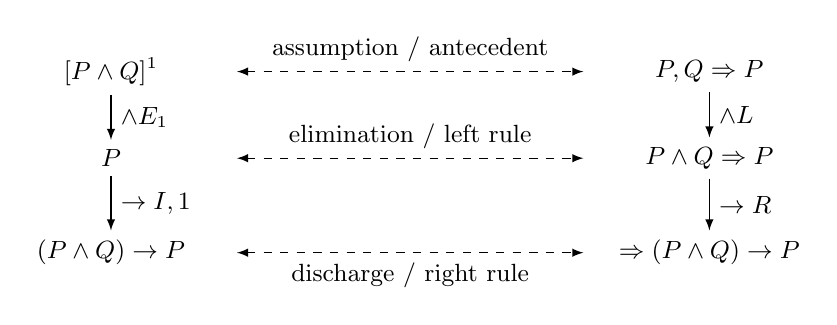
\begin{tikzpicture}[font=\small,>=latex]
  \node (nda) at (-3.8,2.3) {$[P\land Q]^1$};
  \node (ndp) at (-3.8,1.2) {$P$};
  \node (ndi) at (-3.8,0) {$(P\land Q)\to P$};
  \draw[->] (nda) -- node[right] {$\land E_1$} (ndp);
  \draw[->] (ndp) -- node[right] {$\to I,1$} (ndi);

  \node (lki) at (3.8,2.3) {$P,Q\Rightarrow P$};
  \node (lka) at (3.8,1.2) {$P\land Q\Rightarrow P$};
  \node (lkr) at (3.8,0) {$\Rightarrow(P\land Q)\to P$};
  \draw[->] (lki) -- node[right] {$\land L$} (lka);
  \draw[->] (lka) -- node[right] {$\to R$} (lkr);

  \draw[<->,dashed] (-2.2,2.3) -- node[above] {assumption / antecedent} (2.2,2.3);
  \draw[<->,dashed] (-2.2,1.2) -- node[above] {elimination / left rule} (2.2,1.2);
  \draw[<->,dashed] (-2.2,0) -- node[below] {discharge / right rule} (2.2,0);
\end{tikzpicture}
\caption{One natural-deduction/\(\mathsf{LK}\) correspondence (A-117).
The arrows exhibit this example's matching steps; they do not claim a
step-for-step equivalence for arbitrary proofs.}
\label{fig:p02-nd-lk-correspondence}
\end{figure}

\subsection{Analytic tableaux}
\label{sec:p02-analytic-tableaux}

\begin{hbdefinition}{def:p02-cpl-tableau}{Tableau}
For finite \(\Gamma\subseteq\mathsf{Fm}_{\mathsf{CPL}}\), a
\emph{tableau rooted at \(\Gamma\)} is a finite tree of retained branch
lists.  They are built under registry sheet
\hyperref[sheet:tableaux-cpl]{\texttt{sheet:tableaux-cpl}}.  Applying an
expansion appends formulas and marks the principal occurrence as expanded;
it never consumes that occurrence.  A branch is \emph{closed} when it
contains \(\bottom\) or contains both \(\alpha\) and \(\neg\alpha\), and
\emph{open} otherwise.  It is \emph{saturated} when every expandable
occurrence on it is marked.  These marks are metalinguistic bookkeeping, not
formula symbols.  A tableau is closed exactly when every branch is closed.
\end{hbdefinition}

\begin{hbtheorem}{thm:p02-tableau-adequacy}{cited=Smullyan1968}{Tableau adequacy}
Let \(\Gamma\) be a finite set of propositional formulas.  Every closed
tableau rooted at \(\Gamma\) certifies that \(\Gamma\) is unsatisfiable.
Exhaustively expanding unmarked compound occurrences terminates in a finite
saturated tableau.  From any open saturated branch \(B\), define a valuation
by assigning a propositional variable \(p\) true exactly when \(p\) occurs
on \(B\) (and false otherwise).  This branch valuation satisfies every
formula on \(B\), hence every member of \(\Gamma\).  Consequently an
exhaustively expanded saturated tableau has an open branch
exactly when \(\Gamma\) is satisfiable, and it is closed exactly when
\(\Gamma\) is unsatisfiable.
\end{hbtheorem}

\begin{figure}[htbp]
\centering
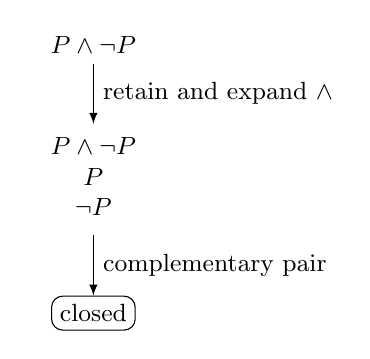
\begin{tikzpicture}[font=\small,>=latex]
  \node (root) at (0,2.7) {$P\land\neg P$};
  \node (expanded) at (0,1.0)
    {$\begin{array}{c}P\land\neg P\\ P\\ \neg P\end{array}$};
  \node[draw,rounded corners,inner sep=3pt] (closed) at (0,-0.7) {closed};
  \draw[->] (root) -- node[right] {retain and expand \(\land\)} (expanded);
  \draw[->] (expanded) -- node[right] {complementary pair} (closed);
\end{tikzpicture}
\caption{A closed propositional tableau for
\(\{P\land\neg P\}\) (A-120).  The root formula remains on the branch
after expansion; the last node records closure rather than replacing any
formula.}
\label{fig:p02-closed-tableau}
\end{figure}

\begin{landscape}
\subsection{Proof-system comparison}
\label{sec:p02-proof-system-comparison}

\begingroup\scriptsize\setlength{\tabcolsep}{3pt}
\begin{longtable}{@{}p{.72in}p{1.20in}p{1.80in}p{1.45in}p{1.70in}@{}}
\caption{Classical propositional proof systems side by side (A-031).}
\label{tab:p02-proof-systems}\\
\toprule
System & Registry home & Derivation object and rule families & Adequacy form & Proof-search behavior \\ \midrule
\endfirsthead
\toprule
System & Registry home & Derivation object and rule families & Adequacy form & Proof-search behavior \\ \midrule
\endhead
Hilbert & \hyperref[sheet:hilbert-cpl]{\texttt{sheet:hilbert-cpl}} & Finite formula sequence; axiom schemas and one inference rule & Sound and complete after the displayed translation, Theorem~\ref{thm:p02-calculi-derivability-equivalence} & Compact for metatheory; little goal-directed structure \\
Natural deduction & \hyperref[sheet:nd-cpl]{\texttt{sheet:nd-cpl}} & Rooted formula tree; introduction, elimination, and nonvacuous discharge & Sound and complete, same theorem & Goal-directed introductions; eliminations may create detours \\
\(\mathsf{LK}\) & \hyperref[sheet:lk]{\texttt{sheet:lk}} & Tree of finite-multiset sequents; initial, structural, logical, and Cut inferences & Sound and complete, same theorem & Backward search becomes analytic when Cut is excluded; normalization is Part~7 \\
Tableau & \hyperref[sheet:tableaux-cpl]{\texttt{sheet:tableaux-cpl}} & Retained branch lists with linear and splitting expansions & Exhaustive saturated tableau closed iff unsatisfiable; open branch yields a model & Direct refutation search with branch closure and countermodel extraction \\
Resolution & \hyperref[sheet:resolution-cpl]{\texttt{sheet:resolution-cpl}} & Clause sequence generated from inputs by binary resolution & Sound and refutationally complete, Theorems~\ref{thm:p02-resolution-soundness} and~\ref{thm:p02-resolution-completeness} & Saturation/search depends strongly on clause choice and redundancy control \\
\bottomrule
\end{longtable}
\endgroup
\end{landscape}
